\documentclass[tikz,border=6pt]{standalone}
\usepackage{lmodern}
\usepackage[T1]{fontenc}
\usepackage{amssymb}
\usetikzlibrary{arrows.meta,shapes.geometric,fit,backgrounds,calc,positioning}
\definecolor{letterA}{HTML}{1F5FA9}
\definecolor{letterB}{HTML}{B5651D}
\definecolor{order}{HTML}{8A9099}
\definecolor{boxline}{HTML}{B9BEC4}
\definecolor{boxfill}{HTML}{F4F5F7}
\definecolor{frozen}{HTML}{E9EEF6}
\definecolor{ref}{HTML}{A6ADB4}
\definecolor{ink}{HTML}{222629}
\tikzset{
  % ---- classes and machines -------------------------------------
  cls/.style        = {circle, draw=ink, line width=.5pt, fill=white,
                       inner sep=0pt, minimum size=13mm, align=center,
                       font=\small},
  committed/.style  = {cls, double, double distance=1pt},
  entry/.style      = {draw=ink, line width=.8pt, -{Stealth[length=1.8mm]}},
  % ---- layers ----------------------------------------------------
  layerbox/.style   = {rounded corners=3pt, draw=boxline, fill=boxfill,
                       line width=.7pt},
  frozenbox/.style  = {layerbox, fill=frozen},
  layertag/.style   = {font=\scriptsize, text=ink, align=left,
                       inner sep=2pt},
  layername/.style  = {font=\scriptsize\bfseries, text=order},
  rorder/.style     = {draw=order, line width=2.2pt,
                       -{Stealth[length=3.2mm,width=3mm]}, opacity=.75},
  % ---- alphabet --------------------------------------------------
  ea/.style         = {draw=letterA, text=letterA, line width=.9pt,
                       -{Stealth[length=2mm]}},
  eb/.style         = {draw=letterB, text=letterB, line width=.9pt,
                       dashed, dash pattern=on 2.4pt off 1.6pt,
                       -{Stealth[length=2mm]}},
  eall/.style       = {draw=ink, text=ink, line width=.9pt,
                       -{Stealth[length=2mm]}},
  elab/.style       = {font=\scriptsize, inner sep=1.5pt,
                       fill=white, fill opacity=.85, text opacity=1},
  % ---- recursion panels ------------------------------------------
  dgnode/.style     = {circle, draw=ink, fill=white, line width=.5pt,
                       inner sep=0pt, minimum size=6.5mm,
                       font=\scriptsize},
  dgleaf/.style     = {dgnode, fill=boxfill, draw=order},
  treeedge/.style   = {draw=ink, line width=.4pt, opacity=.55},
  dagedge/.style    = {draw=ink, line width=.6pt, -{Stealth[length=1.6mm]}},
  refedge/.style    = {draw=ref, line width=.35pt, densely dotted,
                       -{Stealth[length=1.4mm]}},
  emult/.style      = {font=\tiny, text=ref, inner sep=1pt, fill=white},
  elide/.style      = {font=\scriptsize, text=ink, align=center},
  panelcap/.style   = {font=\scriptsize, text=ink, align=center},
}

\begin{document}
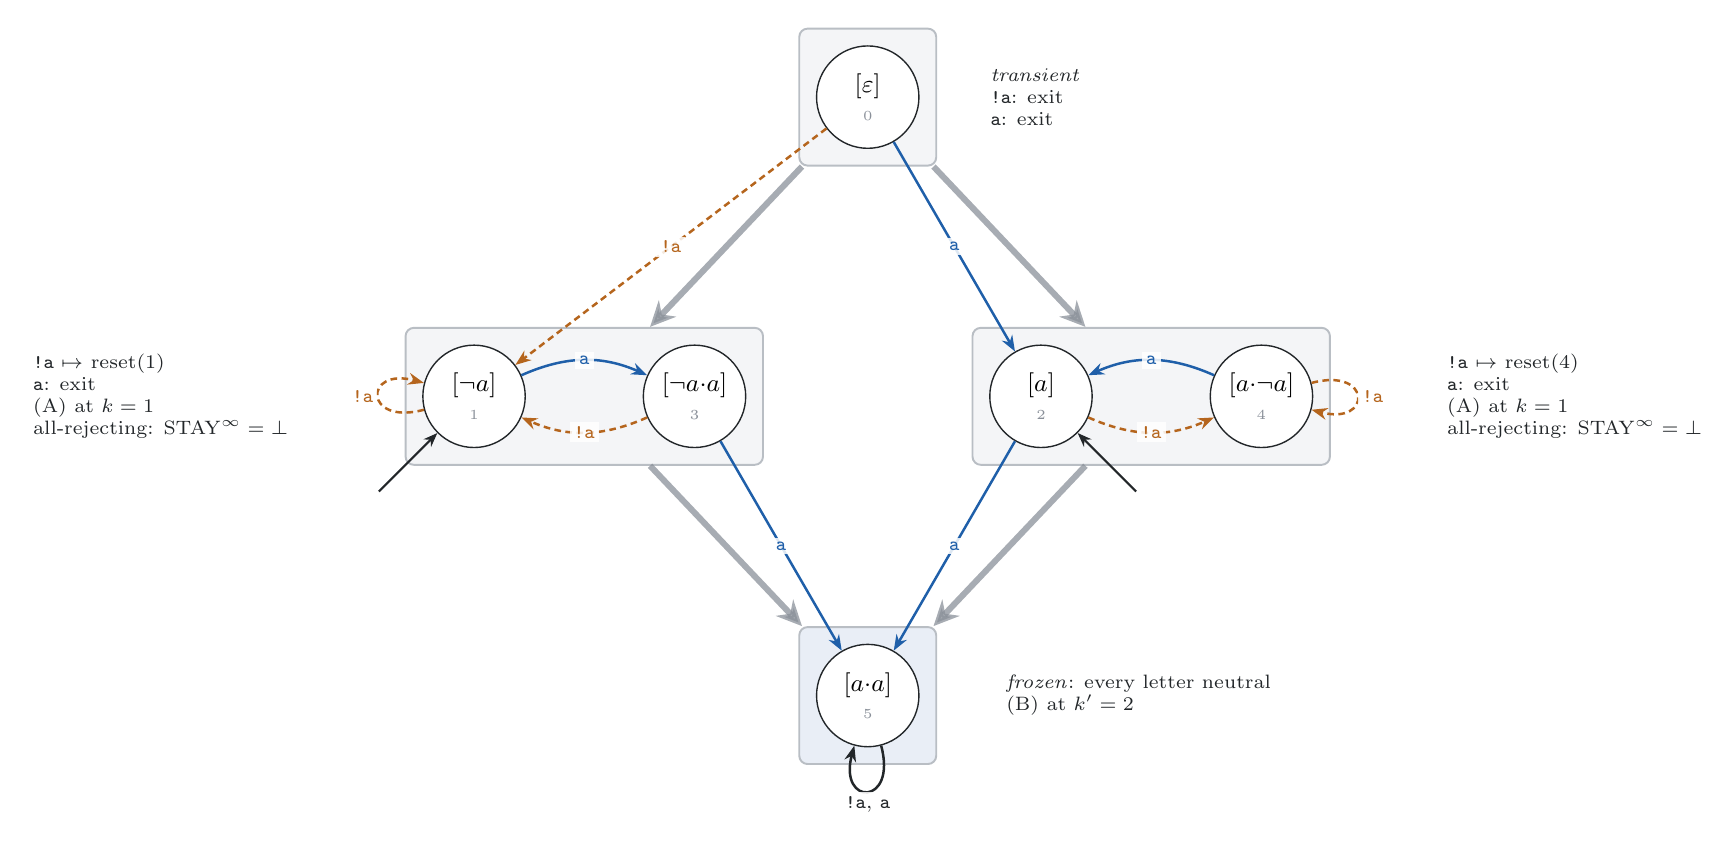
\begin{tikzpicture}
\begin{scope}[scale=1.0]
  \node[cls] (c0) at (0.00,0.00) {$[\varepsilon]$\\[-1pt]\textcolor{order}{\tiny 0}};
  \node[cls] (c1) at (-5.00,-3.80) {$[\lnot a]$\\[-1pt]\textcolor{order}{\tiny 1}};
  \node[cls] (c2) at (2.20,-3.80) {$[a]$\\[-1pt]\textcolor{order}{\tiny 2}};
  \node[cls] (c3) at (-2.20,-3.80) {$[\lnot a {\cdot} a]$\\[-1pt]\textcolor{order}{\tiny 3}};
  \node[cls] (c4) at (5.00,-3.80) {$[a {\cdot} \lnot a]$\\[-1pt]\textcolor{order}{\tiny 4}};
  \node[cls] (c5) at (0.00,-7.60) {$[a {\cdot} a]$\\[-1pt]\textcolor{order}{\tiny 5}};
  \draw[entry] ([shift=(225:1.05)]c1.225) -- (c1.225);
  \draw[entry] ([shift=(315:1.05)]c2.315) -- (c2.315);
  \draw[eb] (c0) to node[elab] {\texttt{!a}} (c1);
  \draw[ea] (c0) to node[elab] {\texttt{a}} (c2);
  \draw[eb] (c1) edge[loop left,looseness=6] node[elab] {\texttt{!a}} (c1);
  \draw[ea] (c1) to[bend left=24] node[elab] {\texttt{a}} (c3);
  \draw[eb] (c2) to[bend left=-24] node[elab] {\texttt{!a}} (c4);
  \draw[ea] (c2) to node[elab] {\texttt{a}} (c5);
  \draw[eb] (c3) to[bend left=24] node[elab] {\texttt{!a}} (c1);
  \draw[ea] (c3) to node[elab] {\texttt{a}} (c5);
  \draw[ea] (c4) to[bend left=-24] node[elab] {\texttt{a}} (c2);
  \draw[eb] (c4) edge[loop right,looseness=6] node[elab] {\texttt{!a}} (c4);
  \draw[eall] (c5) edge[loop below,looseness=6] node[elab] {\texttt{!a}, \texttt{a}} (c5);
  \begin{scope}[on background layer]
    \node[layerbox, fit=(c0), inner sep=6pt] (L0) {};
  \end{scope}
  \node[layertag, anchor=west, xshift=6.0mm] at (L0.east) {\textit{transient}\\\texttt{!a}: exit\\\texttt{a}: exit};
  \begin{scope}[on background layer]
    \node[layerbox, fit=(c1) (c3), inner sep=6pt] (L1) {};
  \end{scope}
  \node[layertag, anchor=east, xshift=-14.0mm] at (L1.west) {\texttt{!a} $\mapsto$ reset(1)\\\texttt{a}: exit\\(A) at $k=1$\\all-rejecting: $\mathrm{STAY}^\infty = \bot$};
  \begin{scope}[on background layer]
    \node[layerbox, fit=(c2) (c4), inner sep=6pt] (L2) {};
  \end{scope}
  \node[layertag, anchor=west, xshift=14.0mm] at (L2.east) {\texttt{!a} $\mapsto$ reset(4)\\\texttt{a}: exit\\(A) at $k=1$\\all-rejecting: $\mathrm{STAY}^\infty = \bot$};
  \begin{scope}[on background layer]
    \node[frozenbox, fit=(c5), inner sep=6pt] (L3) {};
  \end{scope}
  \node[layertag, anchor=west, xshift=8.0mm] at (L3.east) {\textit{frozen}: every letter neutral\\(B) at $k'=2$};
  \begin{scope}[on background layer]
    \draw[rorder] (L0) -- (L1);
  \end{scope}
  \begin{scope}[on background layer]
    \draw[rorder] (L0) -- (L2);
  \end{scope}
  \begin{scope}[on background layer]
    \draw[rorder] (L1) -- (L3);
  \end{scope}
  \begin{scope}[on background layer]
    \draw[rorder] (L2) -- (L3);
  \end{scope}
\end{scope}
\end{tikzpicture}
\end{document}
